
\section{Prototyping}

At this stage, we have implemented the trading simulation software that has been previously described in the requirements, design, and implementation reports. This section details the usage of this software. We will describe how to compile and run this software and how to interpret its output.

\subsection{Program Entry Point}

We have defined the program's entry point (the main function) in an object called \texttt{TradingSimulation} within the Trading Simulation component. The trading strategies that will be tested, the trading events that will be emitted during the simulation, and the time interval that the simulation will test all need to be defined in the entry point of the program.

At this point, the baseline strategy and a buy-and-hold strategy are the only strategies that have been implemented. The Buy-and-Hold strategy is used to compare the baseline against the S\&P 500 index by tracking the change in value of the index over time. The implementation of the Baseline strategy operates on one stock at a time, so you must define 11 instances of the Baseline strategy (one for each stock). The entry point receives a callback after each trading event, allowing it to track the value of each strategy's portfolio. On each market open event, we output a line to a CSV file with three columns. The first column is the time. The second column is the sum of all 11 Baseline strategy portfolio values. The third column is the S\&P 500 Buy-and-Hold strategy portfolio value. A CSV file is a universally recognized file format that is perfect for performing analysis on our data.

This project does not provide any interface that is exceptionally user-friendly, but we can describe a few things about the code in the program entry point that will aid in customizing the parameters of the simulation.

\subsubsection{Specifying the Simulation Time Range}

Since we are backtesting on old data, we need to specify a time range to run the simulation on. This date is specified in the \texttt{TradingSimulation} program in the \texttt{start} and \texttt{end} values that are passed in the constructor of the \texttt{TradingContext}. These values are constructed using the \texttt{OffsetDateTime} class from Java 8's time library. Therefore, it is easy to read and modify the date and time of the timestamp being passed to the \texttt{TradingContext}.

\subsubsection{Customizing the Trading Events}

The trading event emitters are specified in the \texttt{eventSources} value in the \texttt{TradingSimulation} program. \texttt{eventSources} is a list of event emitters that you can easily modify to add or remove the current defined event emitters. By default, the \texttt{eventSources} value is constructed to contain the \texttt{MarketEventsEmitter}, which sends market open/close events, and the \texttt{MicroblogEventEmitter}, which sends an event for each microblog post.

\subsubsection{Customizing the Trading Strategies}

The trading strategies in the simulation are more complicated to specify than one might expect. Because some strategies only operate on one stock and you need to define several instances of them to cover all 11 stocks, the strategies are specified in a map of the strategy name to a list of strategies. This allows us to easily sum the value of a list of strategies and output a CSV with a header containing the strategy names and rows containing the summed up portfolio values. For example, you can store the 11 instances of the baseline strategy with the key ``Baseline'', and the CSV file will contain a column that corresponds to the summed up portfolio values of these 11 strategies. This allows for a very declarative specification of trading strategies without requiring any modification of the code that writes the CSV.

\subsection{Running a Simulation}

Before you can compile and run our code, you first obtain it from our GitHub repo by using the git command line utility: \texttt{git clone} \path{https://github.com/saurabh/cs4624} \cite{github}. As we explained in the design report, we chose to use the sbt build tool for our project. The code can be compiled by executing \texttt{sbt compile} in the project directory. This will compile all three components. Running a main class in a particular component or subproject can be done by executing a command with the following form: \texttt{sbt ``ProjectName/run-main package.ClassName''}. Therefore, to run the \texttt{TradingSimulation} program, we execute \texttt{sbt ``TradingSimulation/run-main cs4624.trading.TradingSimulation''}.

\subsection{Interpreting the Output}

As stated previously, our program outputs data points for the portfolio values of each strategy at the beginning of every market day. Because this information is output in a CSV file, we can easily import it in a spreadsheet software that is suited to perform analysis on the data. An easy visualization of this data can be made by creating a line graph with the dates on the horizontal axis and the portfolio value on the vertical axis. Each strategy would be a separate series on this graph. This allows you to compare the performance of the strategies throughout the year. See figure~\ref{baselineAndIndexGraph} for an example of this that compares the S\&P 500 index fund with the Baseline strategy.

% Figure - baselineAndIndexGraph
\begin{figure}[h]
  \label{baselineAndIndexGraph}
  \begin{center}
    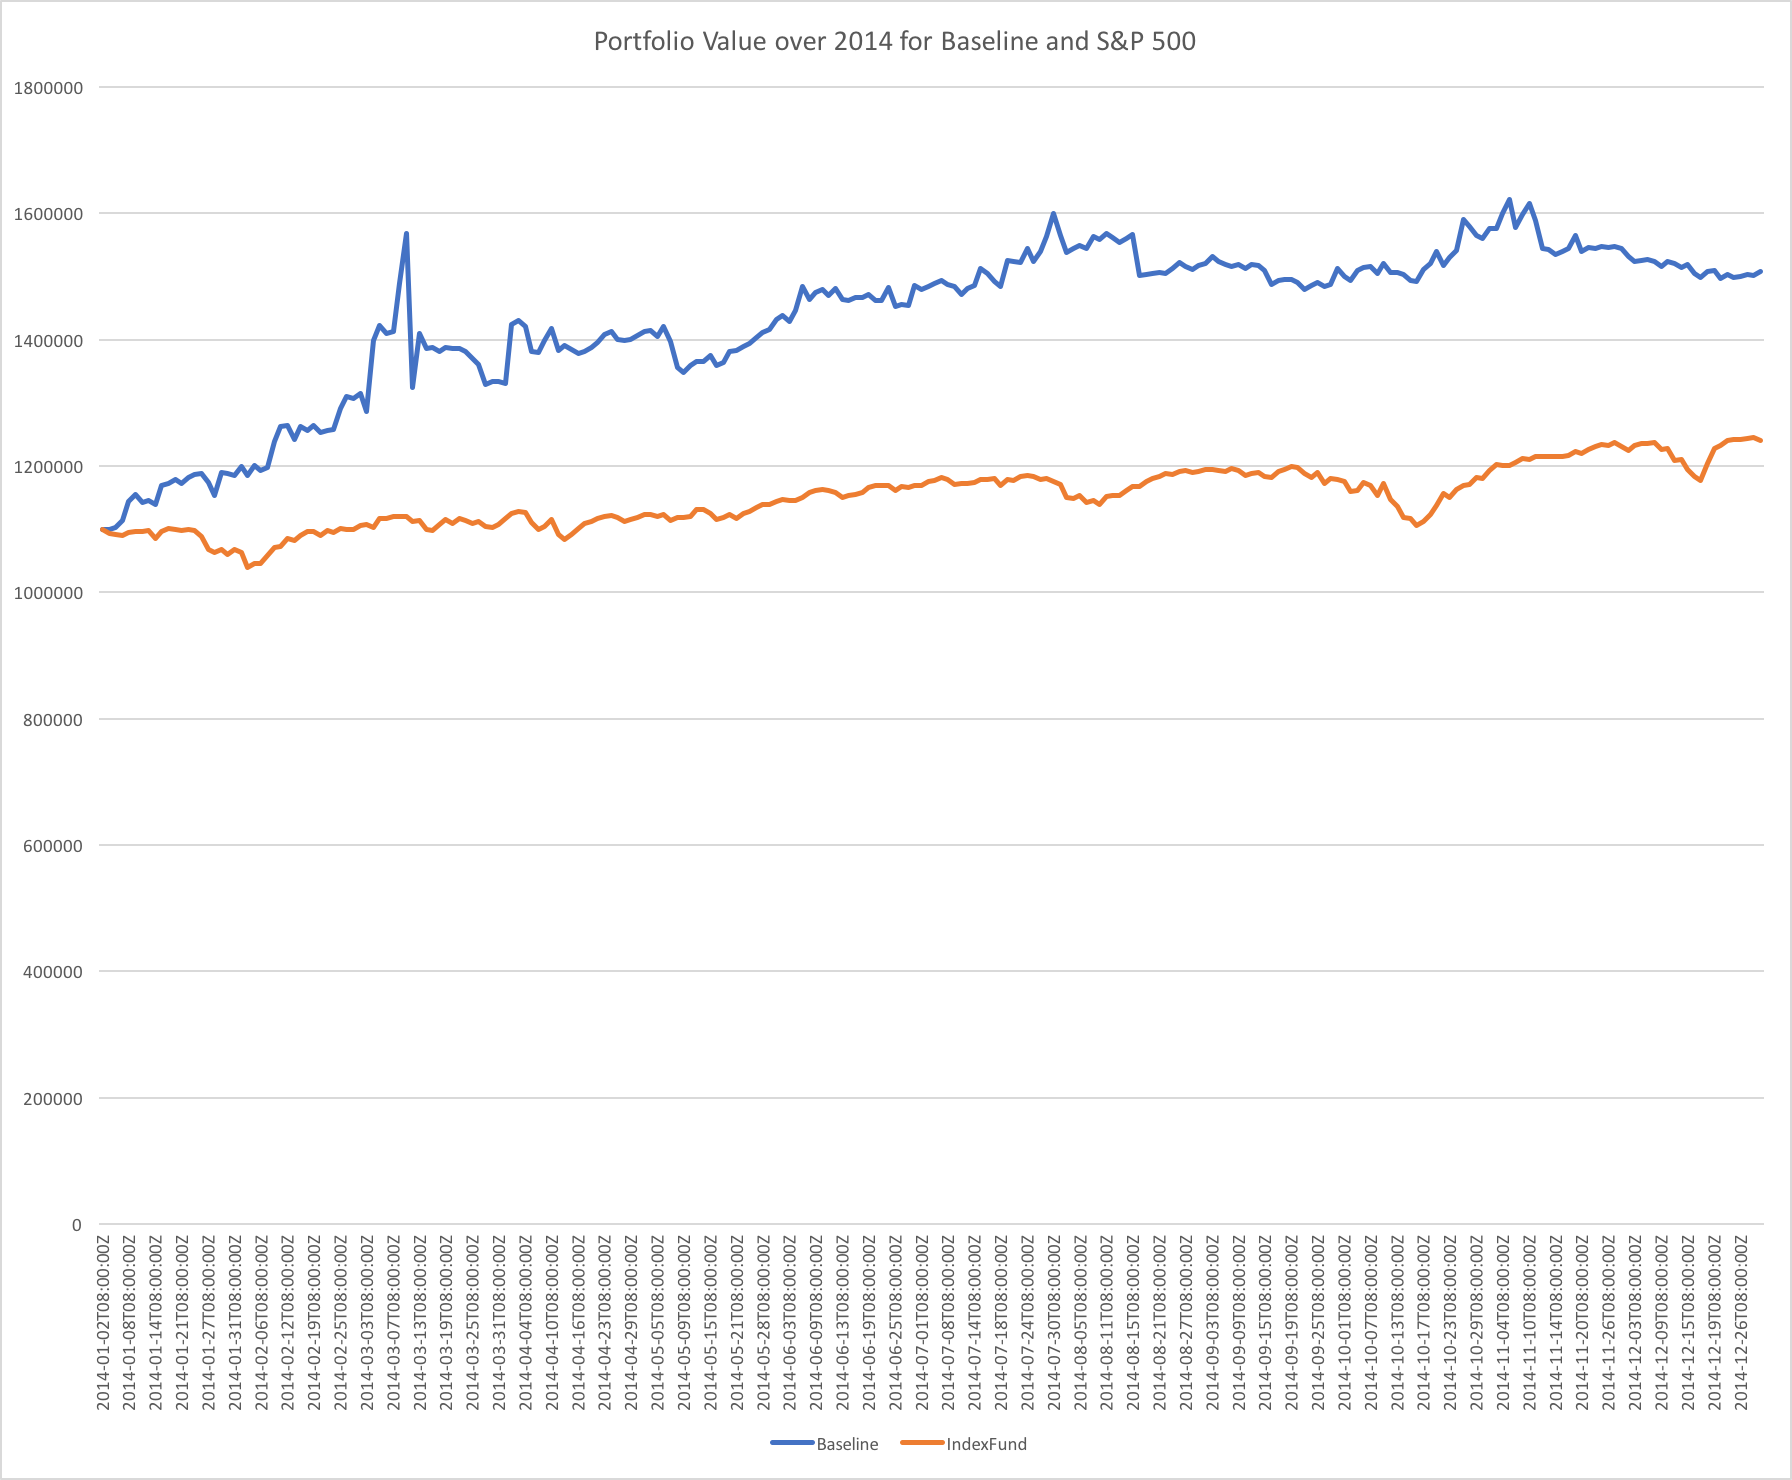
\includegraphics[max width=\textwidth]{baselineAndIndexGraph}
  \end{center}
  \caption{Comparison of the Baseline Strategy and S\&P 500 Index Portfolio Values for the year of 2014.}
\end{figure}

%%% Local Variables:
%%% mode: latex
%%% TeX-master: "../report"
%%% End:
